\section{Numerical Schemes and Simulation}
After establishing that the dynamics of our microscopic model possesses Hamiltonian structure, we can now show these dynamics in action through simulations. In this section we will compare three numerical schemes: explicit Euler, implicit Euler, and Leapfrog, how they are constructed for our model; and how they compare with each other. Furthermore, we construct a solver using the implicit Euler-Maruyama scheme for the stochastic port-Hamiltonian case. For the simulation, the following JuliaLang packages are extensively utilized, \texttt{Agents.jl} and \texttt{DifferentialEquations.jl}.

\subsection{Model Setup}
The simulation is run on a fixed model setup as shown in \autoref{code:model_init}. Here we initialize the values for the number of pedestrians, the extent of the domain in 2D, the desired velocities of the pedestrians, and the parameter values of $\lambda$, $A$, $B$, and $\sigma$.
\begin{table}[H]
    % \centering
    \begin{tabular}{lc}
        Pedestrian Sensitivity: & $\lambda = 2$ \\
        Desired Speed: & $|u| = 1$ \\
        Repulsion Strength: & $A = 5$ \\
        Interaction Range: & $B = 0.3$ \\
        Volatility: & $\sigma = 0.0$
    \end{tabular}
\end{table}
These parameter values are chosen to replicate the results from \cite{tordeux2022multi}, which follows the works of \cite{helbing1995social,tordeux2016collision}. For the stochastic case, we replicate the results from \cite{khelfa2021initiating}. The volatility coefficient $\sigma$ is only relevant for stochastic cases -- as we will see in later sections, whereas in deterministic cases it remains zero.

\begin{listing}[H]
\begin{minted}[escapeinside=??,frame=single, fontsize=\small]{julia}
properties = Dict(
    :?\textlambda? => 2, 
    :A => 5,
    :B => 0.3, 
    :dt => 0.01,
    :?\textsigma? => 0.0,
    :Hamiltonian => 0.0,
    :dH => 0.0
)
number_of_peds = 32 # number of pedestrians
x_len = 11 # domain length in x
y_len = 5 # domain length in y
seed = 42
model = initialize(number_of_peds, x_len, y_len, leapfrog_step, properties,
                   seed)
\end{minted}
\caption{Initialization of the model}
\label{code:model_init}
\end{listing}
The \texttt{initialize} function shown in \autoref{code:model_init} initializes the model with the given parameters. It also utilizes the functionalities provided by the \texttt{Agents.jl} package shown in \autoref{code:model_param} such as \texttt{ContinuousSpace} and \texttt{StandardABM}.
\begin{listing}[H]
\begin{minted}[escapeinside=??, frame=single, fontsize=\small]{julia}
space = ContinuousSpace((x_len, y_len); periodic = true)
model = StandardABM(
    Pedestrian,
    space;
    model_step! = (model) -> model_step!(model, num_solver),
    properties,
    rng # random number generator
)
\end{minted}
\caption{Inside the \texttt{initialize} function from \autoref{code:model_init}, showing that \texttt{ContinuousSpace} method takes care of the space as well as the periodic boundaries}
\label{code:model_param}
\end{listing}


The argument \texttt{num\_solver} is used to specify an ODE solver. As an example \autoref{code:model_init} uses \texttt{leapfrog\_step} from \autoref{code:leapfrog} as a solver. The construction of which is discussed in \autoref{section:numerical_schemes}. Additionally, one can construct other methods to be used in place of \texttt{num\_solver}, such methods can be constructed using the solvers provided by the \texttt{DifferentialEquations.jl} package. These powerful solvers are used for complex scenarios such as solving SDEs (Stochastic Differential Equations) as will be discussed later in this section.

Once the model is initialized, it places the specified number of pedestrians randomly on the grid \autoref{code:agent_init}. Here \texttt{rng} makes use of a Random Number Generator with a specified \texttt{seed} that remains fixed for the model. This is done so that simulation results can be replicated.

\begin{listing}[H]
\begin{minted}[escapeinside=??, frame=single, fontsize=\small]{julia}
for i in 1:number_of_peds
    add_agent!(model;
        pos = [rand(rng)*x_len, rand(rng)*y_len],  # Initial position
        vel = [0.0,0.0], # Initial velocity
        u?\sub{i}? = [1.0,0.0] # uni-directional flow
        # u?\sub{i}? = mod(i,2) == 0 ? [1,0] : [-1,0] # counter_flow
        # u?\sub{i}? = mod(i,2) == 0 ? [0,1] : [1,0] # cross_flow
    )
end
\end{minted}
\caption{Code snippet inside \texttt{initialize}, here every pedestrian is initialized with a position in the space and a desired velocity (\texttt{u}\sub{i}). It can be seen that we can customize the desired velocities to initiate counter flow and cross flow. }
\label{code:agent_init}
\end{listing}

We can also now define a \texttt{model\_step!} function \autoref{code:model_step} that can be used to run our model. At each time-step of the simulation this \texttt{model\_step} takes in the results of the solver used for every agent and modifies the values of each agent. It also calculates the Hamiltonian and its time derivative at each step which are defined in \autoref{section:calc_ham}
\begin{listing}[H]
\begin{minted}[escapeinside=??, frame=single, fontsize=\small]{julia}
function model_step!(model,num_solver)
    for agent in allagents(model)
        v, p = num_solver(agent,model)
        p = normalize_position(p,model) # for periodic boundaries
        agent.vel = v
        agent.pos = p
    end
    model.hamiltonian = calc_hamiltonian(model)
    model.dH = calc_dH(model)
end
\end{minted}
\caption{At each step simulation of the model, \texttt{model\_step!} updates the model parameters as well as the agent parameters.}
\label{code:model_step}
\end{listing}


\subsection{Construction of Numerical Schemes}
\label{section:numerical_schemes}

It is well-established that the preferred numerical methods for Hamiltonian systems are the symplectic methods. These methods are designed such that they preserve the Hamiltonian structure, in other words, they take into account the conservation of energy and hence are better to suited to solve physical systems.

For every pedestrian $i$, the numerical schemes solve for two equations: the positions $q^{k+1}$ and velocities $p^{k+1}$ at time-step $\delta \text{t}$. We recall our dynamic equations from \autoref{eq:micro}, however we write it a bit differently.
\begin{gather}
    \begin{aligned}
    \dot p_i &= a(q_i,p_i) \\
    \dot q_i &= p_i
    \end{aligned}
    \label{eq:diff_pq}
\end{gather}
For clarity, we emphasize the acceleration function and denote it as $a_i(q,p)$ \autoref{eq:acc}. We use this representation to illustrate the numerical methods used.
\begin{equation}
    a_i(q,p) = \lambda(u_i - p_i) - \sum_{j \neq i} \nabla U(q_i - q_j)
    \label{eq:acc}
\end{equation}
In \autoref{code:acc} we define the acceleration function, however we first construct a function \texttt{dU} in \autoref{code:dU} to calculate an interaction potential given the positions \texttt{(pos1, pos2)} of a pair of pedestrians, this is needed in the second term of \autoref{eq:acc}, which sums all interaction potentials given the pedestrian $i$.
\begin{listing}[H]
\begin{minted}[escapeinside=??, frame=single, fontsize=\small]{julia}
function dU(pos1, pos2, model)
    A = abmproperties(model)[:A]
    B = abmproperties(model)[:B]
    dist = euclidean_distance(pos1, pos2, model)
    result = ((get_direction(pos1,pos2,model))/dist)*A*exp(-dist/B)
    return result
end
\end{minted}
\caption{Calculation of \texttt{dU} from \autoref{eq:def_U}. The \texttt{properties} defined in \autoref{code:model_param} can be extracted using \texttt{abmproperties}. The methods \texttt{euclidean\_distance}, and \texttt{get\_direction} are also from \texttt{Agents.jl}}
\label{code:dU}
\end{listing}

\begin{listing}[H]
    \begin{minted}[escapeinside=??, frame=single, fontsize=\small]{julia}    
function acc(pos::SVector{2,Float64}, vel::SVector{2,Float64}, agent, model)
    ?\textlambda? = abmproperties(model)[:?\textlambda?]
    val = ?\textlambda?.*(agent.u?\sub{i}? - vel) - 
          sum(
            dU(pos,i.pos,model) for i in allagents(model) 
            if i.id != agent.id
            )
    return val
end
\end{minted}
\caption{Implementation of \autoref{eq:acc}. The \texttt{allagents} function returns an iterator over all pedestrians in the model}
\label{code:acc}
\end{listing}
The numerical schemes can be a combination of different schemes for each of these equations. The methods used here are:
\begin{itemize}
    \item Explicit/Explicit Euler scheme:
    \begin{gather}\begin{aligned}
        p^{k+1} &= p^k + \delta\text{t} \; a(q^k,p^k) \\
        q^{k+1} &= q^k + \delta\text{t} \; p^k 
    \end{aligned}
    \label{eq:explicit_euler}
    \end{gather}
    \item Implicit/Implicit Euler scheme:
    \begin{gather}
        \begin{aligned}
        p^{k+1} &= p^k + \delta\text{t} \; a(q^{k+1},p^{k+1}) \\
        q^{k+1} &= q^k + \delta\text{t} \; p^{k+1}
    \end{aligned}
    \label{eq:impliict_euler}
    \end{gather}
    Given that this is an implicit method, i.e. $p^{k+1}$ exists on both the right and left side of the equation, $p^{k+1} = p^k + \delta\text{t} \; a(q^{k+1},p^{k+1})$ needs to be solved numerically for each time-step $\delta$t. 
    \item Leapfrog scheme:
    \begin{gather*}\begin{aligned}
        p^{k+1} &= p^k + \dfrac{\delta\text{t}}{2} \; \left(a(q^{k},p^{k})+a(q^{k+1},p^{k+1})\right) \\
        q^{k+1} &= q^k + \delta\text{t} \; p^k + \dfrac{\delta\text{t}^2}{2} \; a(q^{k},p^{k}) 
    \end{aligned}\end{gather*}
    It is to be noted that:
    \begin{equation}
        a(q^{k+1},p^{k+1}) = a(q^{k+1},p^{k}) + \lambda(p^k - p^{k+1})
        \label{eq:acc_relationship}
    \end{equation}
    the leapfrog scheme can be simplified to:
    \begin{gather}\begin{aligned}
        p^{k+1} &= p^k + \dfrac{\delta\text{t}}{2 + \delta\text{t}} \; \left(a(q^k,p^k) + a(q^{k+1},p^{k}) \right) \\
        q^{k+1} &= q^k + \delta\text{t} \; p^k + \dfrac{\delta\text{t}^2}{2} \; a(q^{k},p^{k})
        \label{eq:leapfrog}
    \end{aligned}\end{gather}
\end{itemize}


To demonstrate how these numerical methods are defined in code, we can see the implementation of leapfrog scheme in \autoref{code:leapfrog}. It can be noted that the explicit Euler can be defined similarly because both of these methods (\autoref{eq:explicit_euler} and \autoref{eq:leapfrog}) are explicit.

\begin{listing}[H]
\begin{minted}[escapeinside=??, frame=single, fontsize=\small]{julia}    
function leapfrog_step(agent::Pedestrian, model)
    acc_old = acc(agent.pos, agent.vel, agent, model)
    p = agent.pos + model.dt.*agent.vel + ((model.dt^2)/2).*acc_old
    p = normalize_position(p, model)
    acc_new = acc(p, agent.vel, agent, model)
    v = agent.vel + ((model.dt)/(2 + model.λ*model.dt)).*(acc_old + acc_new)
    return v, p
end 
\end{minted}
\caption{The leapfrog scheme \autoref{eq:leapfrog} in code}
\label{code:leapfrog}
\end{listing}

% \subsection{Using ODE solvers provided by \texttt{DifferentialEquations.jl}}
\textbf{Using ODE solvers provided by \texttt{DifferentialEquations.jl}}

To define implicit Euler method \autoref{eq:impliict_euler}, we make use of the package solvers. As per the directions of \texttt{DifferentialEquations.jl}, we first construct our \texttt{ODEProblem} based on the dynamics provided in \autoref{eq:diff_pq}
\begin{listing}[H]
\begin{minted}[escapeinside=@@, frame=single, fontsize=\small]{julia}    
function ph_model!(du,u,p,t)
    agent, model = p
    vel, pos = u[1:2], u[3:4]
    du[1:2] = acc(agent.pos, agent.vel, agent, model)
    du[3:4] = vel
end
\end{minted}
\caption{Defining \autoref{eq:diff_pq} as an \texttt{ODEProblem}}
\label{code:ph_prob}
\end{listing}

Next we define a solver function that integrates the ODE. Here, we provide the initial conditions \texttt{u0} as the pedestrians velocities and positions, and an integrator function that generates a solution for a single time-step \texttt{dt} using \texttt{step!}. This function can now be used as an argument for \texttt{initialize()} in place of \texttt{num\_solver} in \autoref{code:model_param}.
\begin{listing}[H]
\begin{minted}[escapeinside=@@, frame=single, fontsize=\small]{julia}    
function ode_step(agent, model)
    u0 = [agent.vel[1], agent.vel[2], agent.pos[1], agent.pos[2]]
    tspan = (0.0, Inf)
    p = (agent, model)
    prob = ODEProblem{true}(ph_model!, u0, tspan, p)
    
    # Use the model's integrator
    integrator = init(prob, ImplicitEuler(), dt=model.dt)
    
    # Solve and update agent state
    step!(integrator, model.dt)
    vel = integrator.u[1:2]
    pos = integrator.u[3:4]
    return vel, SVector{2}(pos)
end
\end{minted}
\caption{ODE solver function to solve the model defined in \autoref{code:ph_prob} as \texttt{ODEProblem}. Here, we have chosen the solver as \texttt{ImplicitEuler}}
\label{code:ph_solver}
\end{listing}

Similar to \texttt{ODEProblem} in \autoref{code:ph_solver}, one can also go a step further and define and solve a \texttt{DynamicalODEProblem} or \texttt{SDEProblem} using \texttt{DifferentialEquations.jl}. Since we are also interested in symplectic methods such as the \texttt{leapfrog}, it would also be important to be able to construct a solver for our dynamic problem as well. Here, in contrast to our previous approach, the only difference is that we define the equations for $\dot p$ and $\dot q$ separately, as shown in \autoref{code:ph_dyn_problem}
\begin{listing}[H]
\begin{minted}[escapeinside=@@, frame=single, fontsize=\small]{julia}    
function ph_p!(dv,v,u,p,t)
    agent, model = p
    vel = v[1:2]
    pos = u[1:2]
    dv[1:2] = acc(agent.pos, agent.vel, agent, model)
end
function ph_q!(du,v,u,p,t)
    agent, model = p
    vel = v[1:2]
    du[1:2] = vel
end
\end{minted}
\caption{Defining the \texttt{DynamicalODEProblem} using separate functions for $\dot p$ and $\dot q$}
\label{code:ph_dyn_problem}
\end{listing}
Furthermore, we explicitly separate the initial conditions for velocities and positions, and define the problem using \texttt{DynamicalODEProblem}. We use \texttt{VerletLeapfrog} as our solver as demonstrated in \autoref{code:ph_dyn_solver}.
\begin{listing}[H]
\begin{minted}[escapeinside=@@, frame=single, fontsize=\small]{julia}        
function dynamic_ode_step(agent, model)
    v0 = [agent.vel[1], agent.vel[2]]
    u0 = [agent.pos[1], agent.pos[2]]
    tspan = (0.0, Inf)
    p = (agent, model)
    prob = DynamicalODEProblem(ph_p!,ph_q!,v0,u0, tspan, p)
    
    # Use the model's integrator
    integrator = init(prob, VerletLeapfrog(), dt=model.dt)
    
    # Solve and update agent state
    step!(integrator, model.dt)
    vel = integrator.u[1:2]
    pos = integrator.u[3:4]
    return vel, SVector{2}(pos)
end
\end{minted}
\caption{Solving the model using \texttt{VerletLeapfrog}}
\label{code:ph_dyn_solver}
\end{listing}

This approach of using \texttt{DifferentialEquations.jl} to define and solve our model allows more flexibility to choose from a wider range of sophisticated solvers provided by the package. However, one concerning issue is that this solver uses leapfrog discretization in its original form that will still discretize the model as an implicit scheme, whereas previously, we used the convenient relationship provided by the formulation of the acceleration \autoref{eq:acc_relationship} to manipulate the original discretization to form an explicit leapfrog \autoref{eq:leapfrog}, which proved to be more beneficial as it provides the same results with less computational load.

To solve for the stochastic port-Hamiltonian case, we can make use of an SDE solver. We will first have to define our model as an \texttt{SDEProblem}. To do this, we will define the drift term and diffusion term separately as shown in \autoref{code:sde_problem}. This reflects the standard SDE form as described in \autoref{eq:stoch_micro}.

\begin{listing}[H]
    \begin{minted}[escapeinside=@@, frame=single, fontsize=\small]{julia}        
function ph_stoc_drift!(du,u,p,t)
    agent, model = p
    vel, pos = u[1:2], u[3:4]
    du[1:2] = acc(agent.pos, agent.vel, agent, model)
    du[3:4] = vel
end
function ph_stoc_diffu!(du,u,p,t)
    agent, model = p
    vel, pos = u[1:2], u[3:4]
    @\textsigma@ = model.sigma
    du[1:2] = [@\textsigma@,@\textsigma@] 
    du[3:4] = [0.0,0.0]
end
\end{minted}
\caption{Defining the \texttt{SDEProblem}}
\label{code:sde_problem}
\end{listing}

And finally, we construct our solver to be used as another stepping function for our simulation. It can be seen how the stochastic component is added as a Wiener Process. The solver used for most simulations in the next section is the implicit Euler-Maruyama, however other solvers are also provided the package such as the \texttt{SImplicitMidpoint} \cite{rackauckas2017differentialequations}. This provides room for reassessment on the choice for the solver to be used, specially in a case such as ours that demands symplectic solvers.
\begin{listing}[H]
    \begin{minted}[escapeinside=@@, frame=single, fontsize=\small]{julia}        
function stochastic_ode_step(agent, model)
    u0 = [agent.vel[1], agent.vel[2], agent.pos[1], agent.pos[2]]
    tspan = (0.0, Inf)
    p = (agent, model)
    W = WienerProcess(0.0, 0.0, 0.0)
    prob = SDEProblem(ph_stoc_drift!,ph_stoc_diffu!,u0, tspan, p, noise=W)
    
    # Use the model's integrator
    integrator = init(prob, ImplicitEM(), dt=model.dt)
    
    # Solve and update agent state
    step!(integrator)
    vel = integrator.u[1:2]
    pos = integrator.u[3:4]
    return vel, SVector{2}(pos)
end
\end{minted}
\caption{Solving the SDE using implicit Euler-Maruyama}
\label{code:sde_solve}
\end{listing}

To summarize, in this section we've devised mainly four solvers: for the deterministic port-Hamiltonian model, we have explicit Euler, implicit Euler, and leapfrog; for the stochastic port-Hamiltonian model, we have implicit Euler-Maruyama method. We have allowed ourselves further flexibility by introducing packaged solvers. For the upcoming simulations in the remainder of this section, we will be using \autoref{code:ph_solver} for the implicit Euler as well as explicit Euler by changing the solver to \texttt{Euler}; and \autoref{code:leapfrog} for the leapfrog. Next, we will formulate functions to calculate the Hamiltonian in our model, and then compare the results obtained by each solver.

\subsection{Calculation of Hamiltonian}
\label{section:calc_ham}

To compare these numerical schemes, we can of course observe how the agents interact over time and whether they reach a lane or stripe formation based on the provided desired velocity \texttt{u}\sub{i}. But to have a quantitative measure, we also would like to calculate the Hamiltonian \autoref{eq:Hamiltonian} and observe the change in Hamiltonian \autoref{eq:dH} over time. For this reason we included \texttt{:Hamiltonian} and \texttt{:dH} as key-value pairs in the \texttt{properties} dictionary from \autoref{code:model_init} and define functions \autoref{code:calc_hamiltonian} and \autoref{code:calc_dH} to calculate them.

\begin{listing}[H]
\begin{minted}[escapeinside=??, frame=single, fontsize=\small]{julia}    
function calc_hamiltonian(model)
    kinetic_energy = 0.5.*sum(
        [transpose(a.vel)*a.vel for a in allagents(model)]
        )
    potential_energy = 0.5.*sum(
        [sum_potU(a,allagents(model),model) for a in allagents(model)]
        )
    return kinetic_energy + potential_energy
end
\end{minted}
\caption{Calculation of Hamiltonian $H(z(t))$ as defined in \autoref{eq:Hamiltonian}. For clarity, the kinetic and potential terms are calculated separately. One can easily observe that the function \texttt{sum\_potU} evaluates the double summation.}
\label{code:calc_hamiltonian}
\end{listing}

\begin{listing}[H]
\begin{minted}[escapeinside=??, frame=single, fontsize=\small]{julia}    
function calc_dH(model)
    return sum(
        [model.?\textlambda?*norm(i.vel)*norm(i.u?\sub{i}? - i.vel) for i in allagents(model)]
        )
end
\end{minted}
\caption{Calculation of $\frac{d}{dt}H(z(t))$ as defined in \autoref{eq:dH}}
\label{code:calc_dH}
\end{listing}

Inner summation of the second term in \autoref{eq:Hamiltonian} is defined in the function \texttt{sum\_potU}. This simply adds all the individual potential energies between pairs of all combinations of the pedestrians in the model. The potential energy \autoref{code:sum_potU} is calculated following the definition provided in \autoref{eq:def_potU}
\begin{listing}[H]
\begin{minted}[escapeinside=@@, frame=single, fontsize=\small]{julia}    
function potU(a1::Pedestrian,a2::Pedestrian, model)
    A = model.A
    B = model.B
    dist = euclidean_distance(a1, a2, model)
    return A*B*exp(-dist/B)
end

function sum_potU(a1::Pedestrian, agents, model)
    return sum([i.id != a1.id ? potU(a1, i, model) : 0 for i in agents])
end
\end{minted}
\caption{Evaluating the inner summation of potential energies from \autoref{eq:Hamiltonian} using \texttt{sum\_potU} in the calculation of the Hamiltonian in \autoref{code:calc_hamiltonian}}
\label{code:sum_potU}
\end{listing}

\pagebreak
\subsection{Comparison of Numerical Schemes}
\label{section:compare_num_solvers}
We can now compare the numerical schemes by determining how accurately they are describing the dynamics. This is done by evaluating the error, which is defined as the difference between the time derivative of the Hamiltonian at time-step $k$ and the difference between the Hamiltonian at time step $k$ and $k-1$, resulting in the following expression:
\begin{align}
    \text{Error} &= \dfrac{d}{dt}H(z^k) - \dfrac{1}{\delta \text{t}}\left(H(z^k)) - H(z^{k-1})\right) \nonumber \\ 
    \text{Error} &= \lambda\langle p^k,u-p^k\rangle - \dfrac{1}{\delta \text{t}}\left(H(Q^k, p^k)) - H(Q^{k-1}, p^{k-1})\right)
    \label{eq:error}
\end{align}

The first term of \autoref{eq:error} is the time derivative of the Hamiltonian $\frac{d}{dt}H(z(t))$, the expression of which was already obtained in \autoref{eq:dH}. Since the second term is the approximation of the time derivative, it can be noted that the $\text{Error} \rightarrow 0$ as $\delta \text{t} \rightarrow 0$. 

We concentrate once again to the deterministic port-Hamiltonian case, and run our simulations to compare the following numerical schemes: explicit Euler, implicit Euler, and Leapfrog. Hence, we initialize 3 models each using one of the mentioned solvers. The intent here is to replicate the results obtained from \cite{tordeux2022multi}, hence we use the same model parameters as described in \autoref{code:model_init} and \autoref{code:agent_init}, namely $u_i = [1,0]$ for all pedestrians $i$. The model is run for 20 seconds of simulation time, for each step-size $\delta \text{t}$ ranging from 0.01 to 0.2.


\begin{figure}[H]
    \centering
    \begin{subfigure}{.49\textwidth}
        \centering
        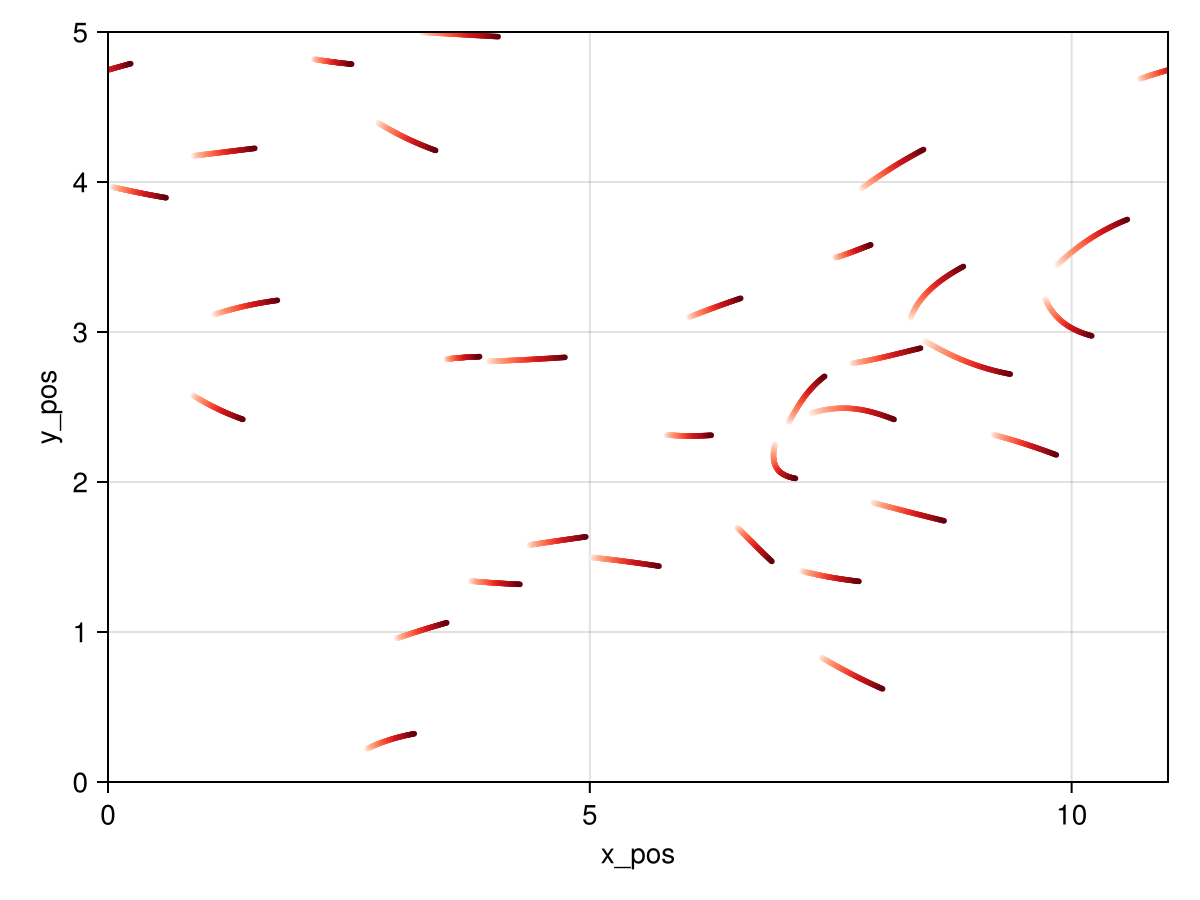
\includegraphics[width=\linewidth]{figures/Uniflowdflow_101.png}
        \caption{Unidirectional flow [start]}
    \end{subfigure}
    \begin{subfigure}{.49\textwidth}
        \centering
        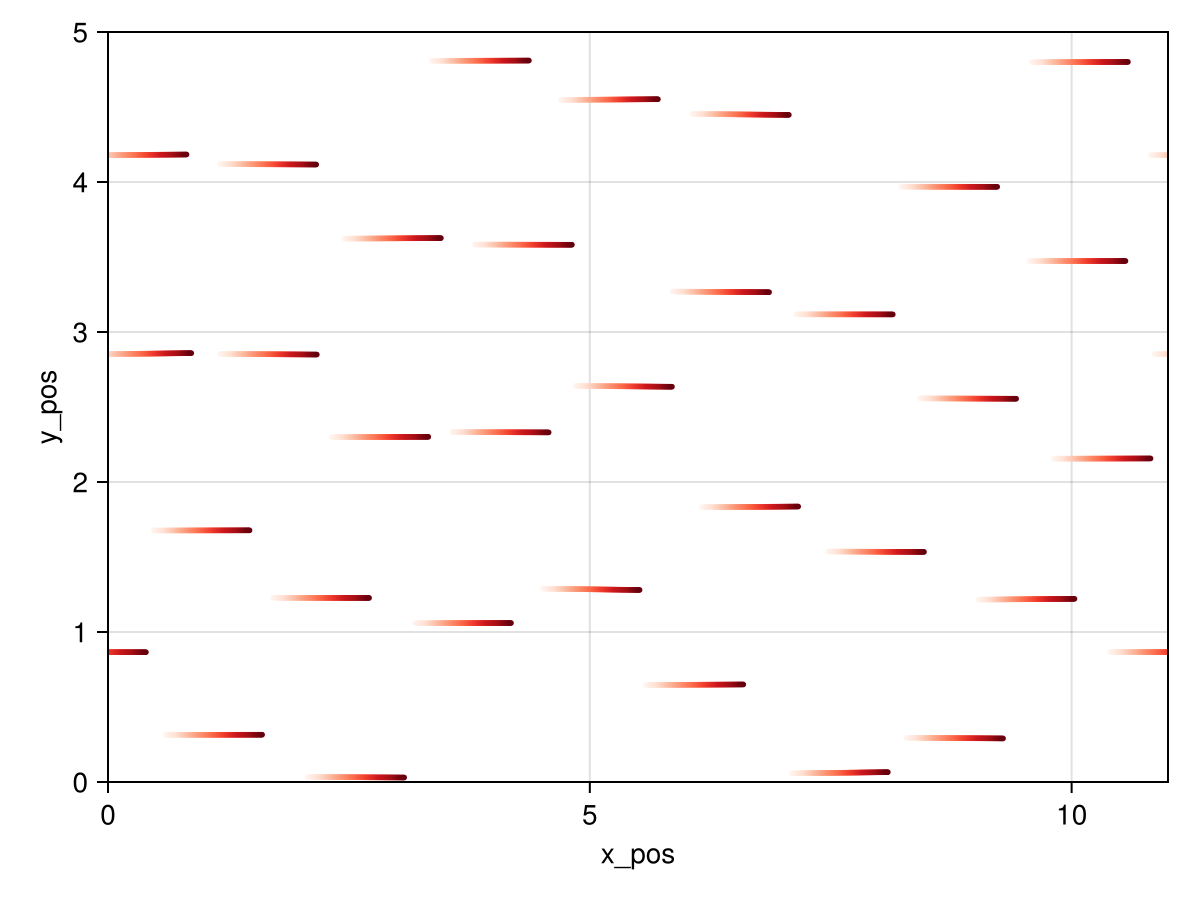
\includegraphics[width=\linewidth]{figures/Uniflowdflow_4000.png}
        \caption{Unidirectional flow [steady-state]}
    \end{subfigure}
    \caption{The progress of the simulation at (a) the start of the simulation and (b) after some time, reaching a steady state}
    \label{plot:uniflow_positions}
\end{figure}

\pagebreak
It can be observed from \autoref{plot:uniflow_positions} how the pedestrians start from a random arrangement and gradually reach a steady state by achieving their desired unidirectional motion.
\begin{figure}[H]
    \centering
    \begin{subfigure}{.49\textwidth}
        \centering
        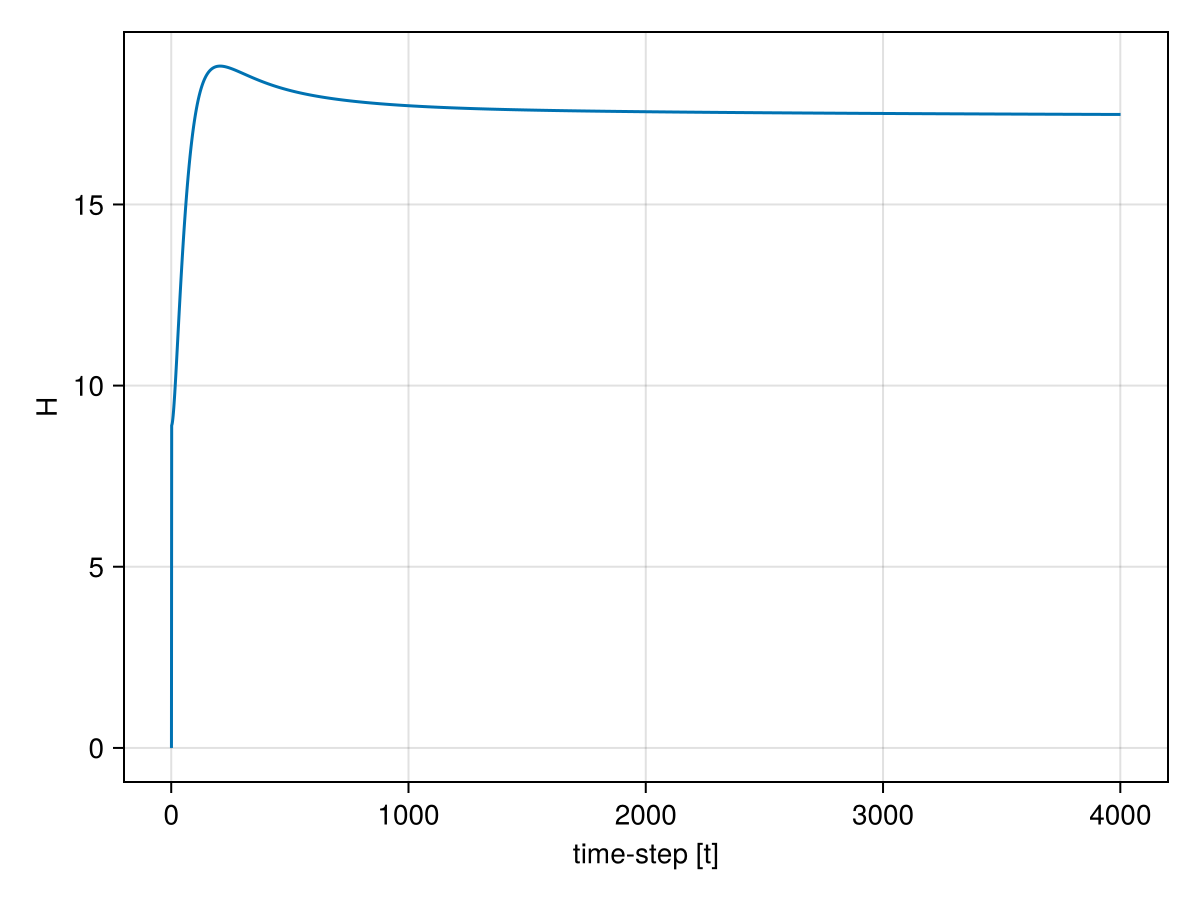
\includegraphics[width=\linewidth]{figures/H_Uniflow.png}
    \end{subfigure}
    \begin{subfigure}{.49\textwidth}
        \centering
        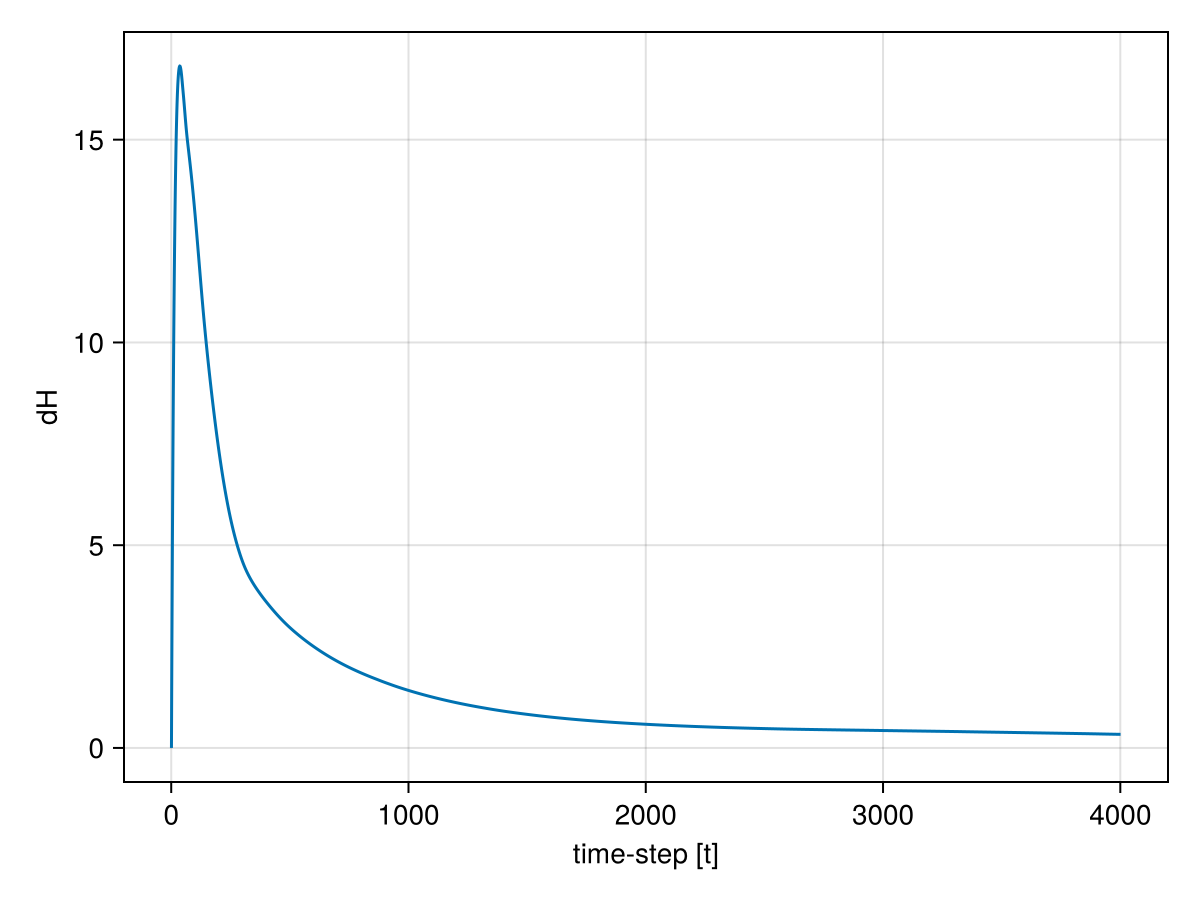
\includegraphics[width=\linewidth]{figures/dH_Uniflow.png}
    \end{subfigure}
    \caption{$H(z(t))$ and $\frac{d}{dt}H$ as the simulation progresses over time.}
    \label{plot:uniflow_hamiltonian}
\end{figure}

As demonstrated in \autoref{plot:uniflow_hamiltonian} the change in Hamiltonian with respect to time, $\frac{d}{dt}H(z(t))$ tends to zero as the system reaches its steady state. Using this solution of the uni-directional flow, we have generated a plot for the errors obtained from each numerical scheme in \autoref{plot:errors}. The plot \autoref{plot:scheme_error} shows the mean errors obtained for solving the model using a numerical scheme with fixed time-steps $\delta \text{t}$, whereas \autoref{plot:scheme_time} illustrates the computation time required to solve the model for fixed time-steps $\delta \text{t}$.

\begin{figure}[H]
    \centering
    \begin{subfigure}{.49\textwidth}
        \centering
        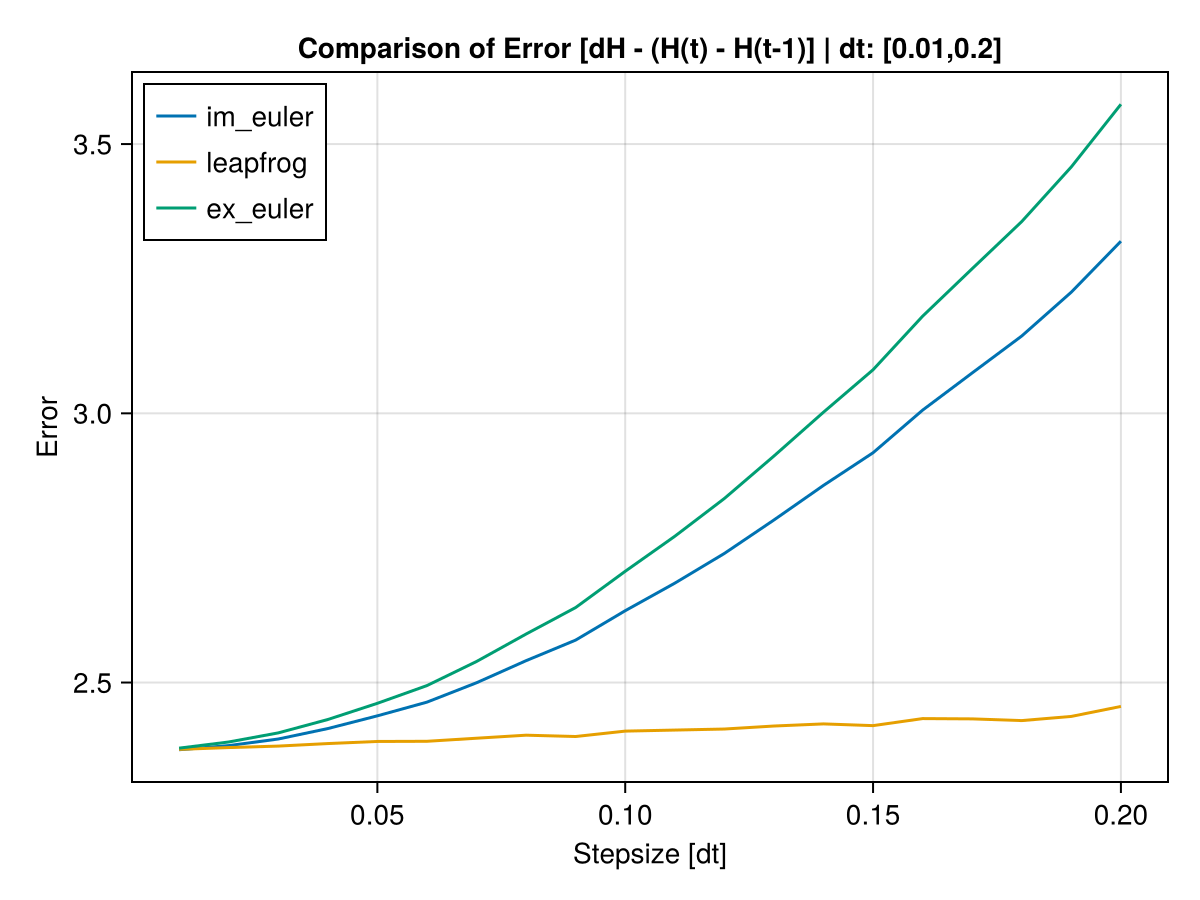
\includegraphics[width=\linewidth]{figures/manual_scheme_error1.png}
        \caption{Mean error of the schemes}
        \label{plot:scheme_error}
    \end{subfigure}
    \begin{subfigure}{.49\textwidth}
        \centering
        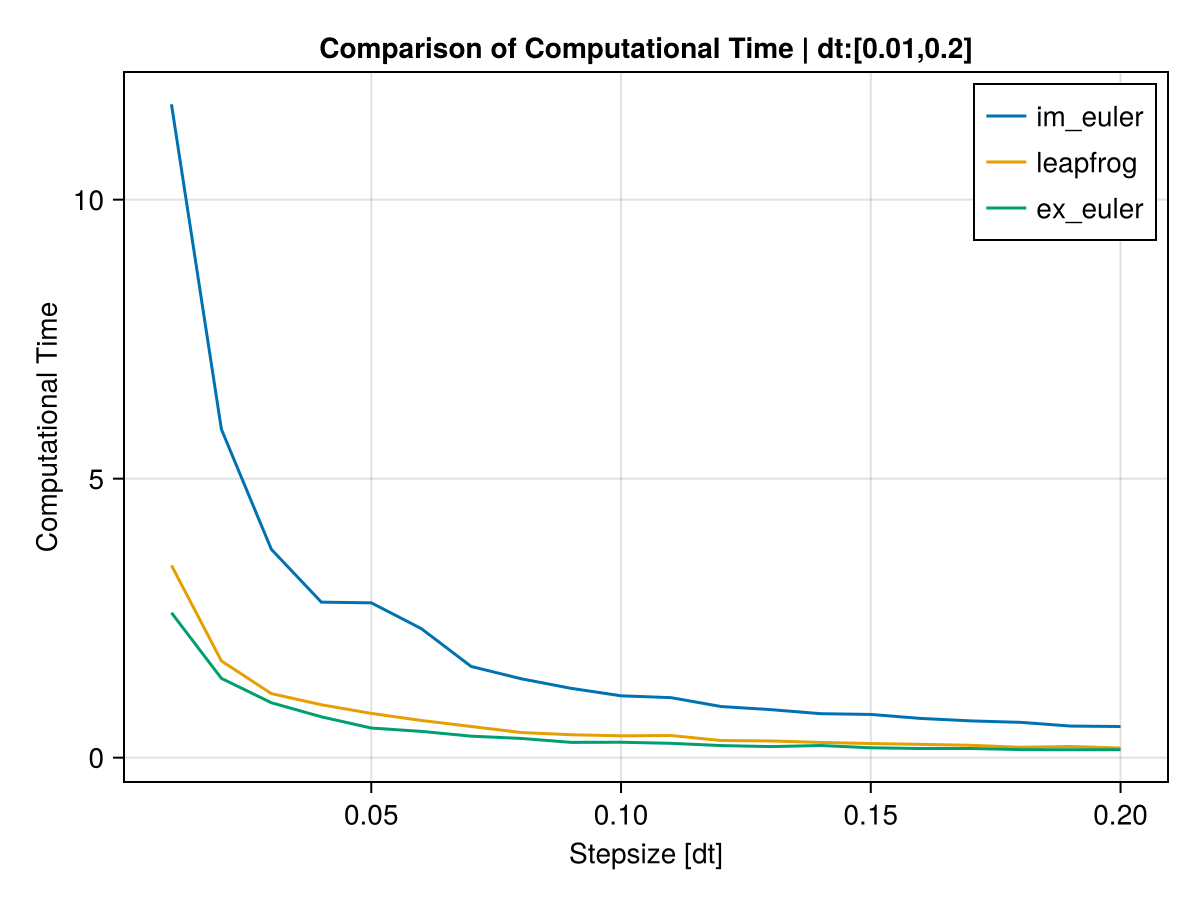
\includegraphics[width=\linewidth]{figures/time1.png}
        \caption{Computation time of the schemes}
        \label{plot:scheme_time}
    \end{subfigure}
    \caption{Comparison of numerical schemes in terms error and computation time}
    \label{plot:errors}
\end{figure}

As one would expect the errors do increase when the $\delta \text{t}$ increases, however the stark contrast between the minute numerical errors of leapfrog scheme to others clearly shows the benefit of using symplectic schemes for solving Hamiltonian systems. The computation time of leapfrog here is similar to that of explicit Euler. Implicit Euler, on the other hand, yields results that are only slightly better than its explicit counterpart regarding errors. Due to its implicit nature, the implicit Euler also requires extra steps to numerically solve equations resulting it to be the most computationally expensive compared to the other two.

With these results in mind, we conclude this section with leapfrog as our choice to be used for all deterministic dynamical models for our simulations in the coming section.
